\section{Communications}
\label{blDOCOM}

For the communications subsystem 5 different topics were investigated:
\begin{itemize}
\item Tracking
\item Swarm satellites crosslink frequency
\item D/L and U/L frequency
\item Antenna configuration
\item Communications architecture
\end{itemize}

\subsection{Tracking}
For tracking there are the following design options:
\begin {itemize}
\item \ac{MANS}
\item \acs{GPS}
\item \ac{TDRS}
\item Satellite crosslinks
\item Ground tracking
\end {itemize}

MANS uses observations of the Earth, Sun and Moon from a single sensor to provide real-time position and attitude data. These objects can be unambiguously identified with high reliability and low cost and observations can be done with minor modifications to attitude sensors already on most spacecrafts. The MANS flight software can also make use of data from a GPS receiver, star sensors, gyros and accelerometers to increase the accuracy. MANS also provides ground point look and Sun direction information and works at any altitude between \acs{LEO} and \acs{GEO}.

GPS is a system of navigation satellites which allows position determination with an accuracy of 50-100m for non-military use. GPS can also be used to determine attitude by using multiple GPS antennas attached to a rigid element of the spacecraft which allows accuracies between 0.3 and 0.5 degrees. There must always be 4 GPS satellites in sight in order for the system to work, but it can not be guaranteed that this number of satellites is in sight continuously.

TDRS is a system of 2 satellites operated by NASA, which can provide tracking data coverage for 85\% to 100\% of most low-Earth orbits. The system collects mostly range and range-data from the TDRS satellite to the satellite being tracked. Angular information is available, but is much less accurate than the range and range-rate data. If atmospheric drag effects on a satellite are small, TDRS can achieve 3$\sigma$ accuracies of 50m which is considerably better than most ground-tracking systems.

Satellite crosslinks allow relative position determinations by use of cross link equipment. If absolute position determination is required a seperate tracking system is required which also can allow relative position determintion, making the satellite crosslinks technique redundant.

Finally ground tracking allows determination of range and range rate, angular measurements are also available at times but are typically far less accurate. Several passes over a ground station are required for orbit determination. 3$\sigma$ accuracies typically are about several kilometers for low-Earth orbit.

\subsection{Swarm satellites crosslink frequency}
The frequency band normally used for inter satellite communications are the V-band frequency. This band lies around 60 GHz and has no limit on the power flux density.

\subsection{D/L and U/L frequency}
Frequency bands available for upload and download of scientific data are:
\begin{itemize}
\item C-Band
\item X-Band
\item Ku-Band
\item Ka-Band
\item SHF/EHF-band
\end{itemize}

Details for all frequency bands can be found in \cite{Larson}, p566.

\subsection{Antenna configuration}
The following antennas, suitable for beamwidths less than 20 degrees, producing gains above 15dB, are considered:
\begin{itemize}
\item Parabolic reflector center-feed
\item Parabolic reflector cassegrain
\item Parabolic reflector off-set feed
\item Phased array
\item Lens with switched-feed array
\item Parabolic reflector off-set shaped subreflector with feed array for scanning
\end{itemize}

Drawings and descriptions of these antennas can be found in \cite{larson}, p 573.

\subsection{Communications architecture}
In this subsection we will discuss the possible communications architectures and the transmission power and bandwidth required for the communication subsystem in each satellite:
\begin{itemize}
\item Centralized architecture
\item Decentralized architecture
\item Extremely decentralized architecture
\end{itemize}

In centralized architecture there is one central satellite which handles all communication between the swarm and the Earth, which means the communication subsystem of the central satellite requires a broad bandwidth and high transmission power both for the communication between itself and the swarm and the Earth.

A decentralized architecture gives all satellites the bandwidth and transmission power to communicate with the ground, but communication within the swarm is also still possible.

In an extremely decentralized architecture all satellites communicate independently to the ground and also communication between the swarm goes through ground.

The design option tree for communications id shown in figure \ref{fig:docom} on page \pageref{fig:docom}.

\begin{figure}
\centering
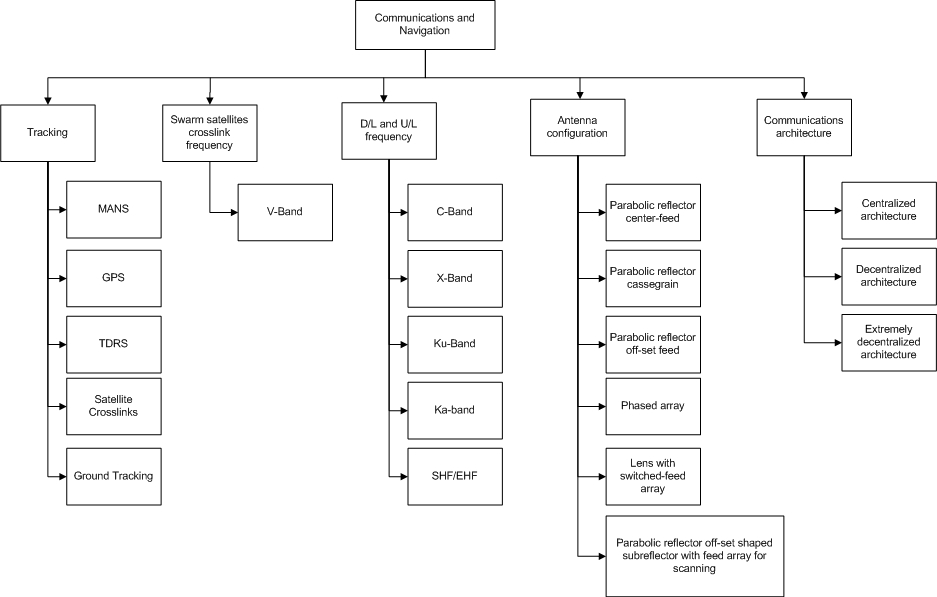
\includegraphics[width=1.0\textwidth, angle=90]{chapters/img/DOTCom.jpg}
\caption{Design option tree for communications}
\label{fig:docom}
\end{figure}